\documentclass[slovene,11pt,a4paper]{article}
%\usepackage{fullpage}
\usepackage[margin=2cm]{geometry}

\usepackage[T1]{fontenc}



%dodatni paketki:
\usepackage{graphicx}
\usepackage{amsmath,amsfonts,amsthm} %matematicni paket
\usepackage{color} % omogoča barvno pisanje
\usepackage[utf8]
{inputenc}
\usepackage[slovene]{babel} % slovenski jezik/hyphenation
\usepackage{hyperref} %naredi vse povezave rečerenc, kazala,...
\numberwithin{equation}{section} % Number equations within sections (i.e. 1.1, 1.2, 2.1, 2.2 instead of 1, 2, 3, 4)
\numberwithin{figure}{section} % Number figures within sections (i.e. 1.1, 1.2, 2.1, 2.2 instead of 1, 2, 3, 4)
\numberwithin{table}{section} % Number tables within sections (i.e. 1.1, 1.2, 2.1, 2.2 instead of 1, 2, 3, 4)
\usepackage{eurosym} %za znak €

\usepackage{mathrsfs}
\usepackage{mathabx} % za kemisjke smeri in naslednje 3 vstrice
\catcode`_=12
\begingroup\lccode`~=`_\lowercase{\endgroup\let~\sb}
\mathcode`_="8000

\usepackage{placeins}
\usepackage[margin=2cm]{geometry}
\usepackage{amsmath}
\usepackage{physics}


\begin{document}
\begin{titlepage}

\newcommand{\HRule}{\rule{\linewidth}{0.5mm}} % Defines a new command for the horizontal lines, change thickness here

\center % Center everything on the page

%----------------------------------------------------------------------------------------
%	LOGO
%----------------------------------------------------------------------------------------

%\includegraphics{Logo}\\[1cm] % Include a department/university logo - this will require the graphicx package
 
%----------------------------------------------------------------------------------------


\includegraphics[width=2cm]{slike/aaa}\\[0.5cm]
 
%----------------------------------------------------------------------------------------
%	NASLOV DELA
%----------------------------------------------------------------------------------------
\textit{Univerza v Ljubljani}\\
\textit{Fakulteta za {\color{red}matematiko in fiziko}}\\[0.5cm]

\emph{Oddelek za fiziko}\\[0.5cm] % Oddelek za fiziko


%----------------------------------------------------------------------------------------
%	TITLE SECTION
%--------------------------------------------------------------------------------------
\HRule \\[0.4cm]
\huge {\bfseries 1. naloga: Numerično reševanje Schrodingerjeve enačbe -2.del}\\[0.4cm] % NASLOV SEMINARJA
\HRule \\[0.5cm] 

 \textsc{\large Poročilo pri predmetu višje računske metode}\\
 \textsc{\large 2016/2017}\\[1cm] % SEMINASKO DELO
 
%----------------------------------------------------------------------------------------
%	AUTHOR SECTION
%----------------------------------------------------------------------------------------



% If you don't want a supervisor, uncomment the two lines below and remove the section above
\Large \emph{Avtor:}\\
Klemen \textsc{Rahne}\\
28152028\\[2cm]
%----------------------------------------------------------------------------------------
%	DATUM
%----------------------------------------------------------------------------------------

{\large \today } \\[0.5cm] % Date, change the \today to a set date if you want to be precise

	

\end{titlepage}


%----------------------------------------------------------------------------------------
%	KAZALO
%----------------------------------------------------------------------------------------

%\tableofcontents

%----------------------------------------------------------------------------------------
%	ZAČETEK TEKSTA
%----------------------------------------------------------------------------------------
\section{Lastne energije}
Iščemo lastne energije kvantnega sistema v harmonskem potencialu z dodatnim anharmonskim členom. Tak sistem bomo reševali v bazi ($\Phi _N(x)$) rešitev nezmotenega harmonskega oscilatorja, ki ima za bazo nasljednje funkcije:
\begin{equation}
\label{ho-resitve}
\Phi _N(x)=\frac{1}{\pi^{\frac{1}{4}}\sqrt{2^N N!}} H_N(x) \exp{(\frac{-x^2}{2})}
\end{equation} 
kjer je $H_N$ Hermitov polinom $N$-te stopnje. Za iskanje lastnih energij harmonskega oscilatorja z dodatnim anharmonskim členom imamo Schroedingerjevo enačbo:
\begin{equation}
\label{sch-osnovna}
\hat{H} \Psi_N = E_N \Psi_N
\end{equation}
Hamiltonov operator lahko zapišemo kot vsoto Hamiltonovega operatorja harmonskega oscilatorja in prispevek anharmonskega člena potenciala:
\begin{equation}
\hat{H}=\hat{H_0}+ \lambda \hat{H'}
\end{equation}
rešitve samo operatorja $H_0$, katere bomo uporabljali kot bazne funkcije so funkcije \ref{ho-resitve}. Z uporabo nastavka:
\begin{equation}
\Psi(x) = \sum _0^N c_N \Phi_N (x)
\end{equation}
Z uporabo variacijskega pristopa se enačba \ref{sch-osnovna} prepiše na problem iskanja lastne vrednosti matrike $H$, ki ima na mestu $i,j$ naslednjo vrednosti:
\begin{equation*}
H_{i,j}= \bra{i} \hat{H} \ket{j}= \bra{i}\hat{H_0} \ket{j} + \lambda \bra{i} \hat{H'} \ket{j} = (i+\frac{1}{2}) \delta_{i,j} + \lambda \bra{i}x^4 \ket{j}; \quad i=0,1,..,N-1
\end{equation*}
Dodatni člen$\bra{i}x^4 \ket{j}$, matriki $H$, doda izven diagonalne elemente.

\begin{figure}[!htb]
\centering
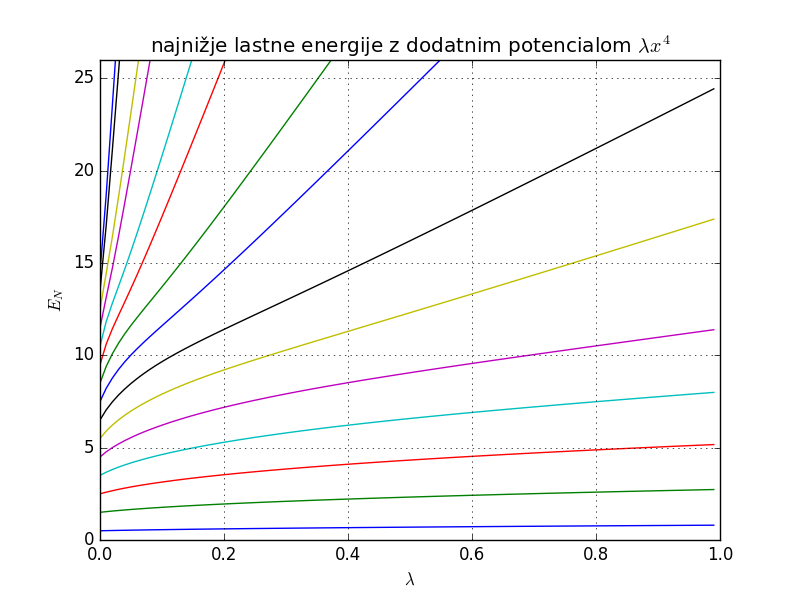
\includegraphics[scale=0.45]{slike/najnizje_energije.png}
%\caption{first figure}


\caption{Najnižje lastne energije v odvisnosti od $\lambda$. Velikost matrike je bilo $15x15$.}
\end{figure}
\newpage
Poglejmo kako vpliva velikost matrike na vrednosti lastnih energij.













\newpage

\section{naloga}
Oglejmo si kako izgleda če osnosvno valovno funkcijo zamaknemo za razdaljo $a$. Pričakovati je, da se valovna funkcija šele po nekaj korakih stabilizirala okoli izhodišča potenciala.


\begin{figure}[!htb]
\centering
\begin{minipage}{0.5\textwidth}
\centering
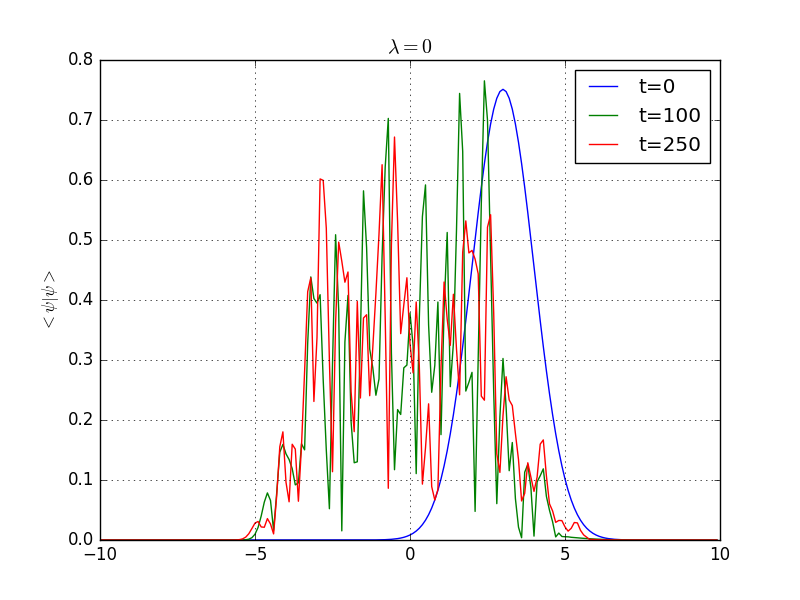
\includegraphics[scale=0.45]{slike/casovni_razvoj_izmika.png}
%\caption{first figure}
\end{minipage}\hfill
\begin{minipage}{0.5\textwidth}
\centering
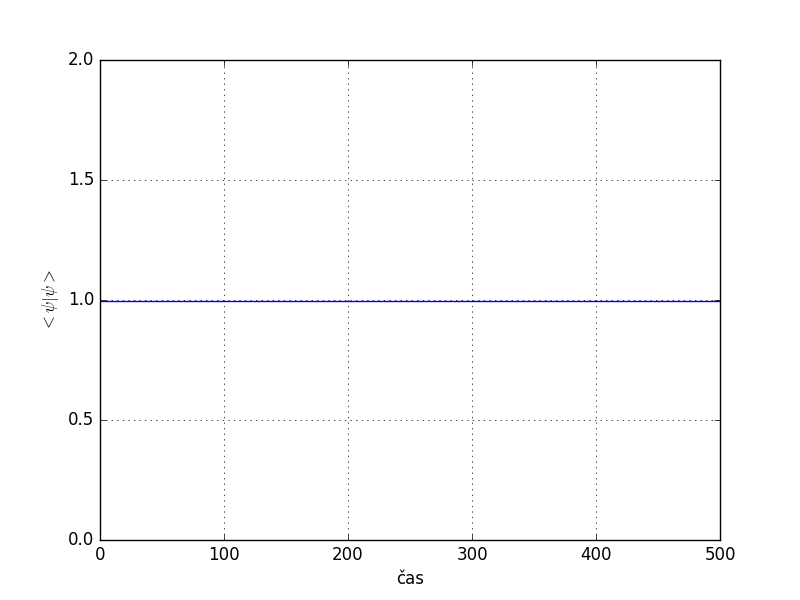
\includegraphics[scale=0.45]{slike/ohranjanje_delcev.png}
%\caption{second figure}
\end{minipage}

\caption{Na levem grafu vidimo časovni potek valovne funkcije po času. Na začetku je funkcija zelo jasno določena, kasneje se pa gaussova oblika "zamaže". Na desnem grafu vidimo, da se kljub zamazanosti gausove krivulje ohranja verjetnostna gostota.}
\end{figure}

\end{document}
